\documentclass[11pt,a4paper,oneside,english]{article}
\usepackage{latexstyles/print}

\title{
	Deliberative Subjectivities on Economic Integration in the European Union\\*
	---\\*
	A Draft Project Proposal for the Europa-Universität Flensburg
	}
\author{
	\href{http://www.maxheld.de}{Maximilian Held}
}
\date{
	\today
}

\addbibresource{../held-library/held_library.bib}
%\graphicspath{/img/}

\begin{document}

\maketitle

\begin{abstract}
	\immediate\write18{pandoc README.md -t latex -o Output/tmp.tex}%
	\input{tmp.tex}
\end{abstract}

\newpage

\epigraph{
	``The Secretary, after mature reflection on this point, entertains a full conviction, that an assumption of the debts of the particular states by the union, and a like provision for them, as for those of the union, will be a measure of sound policy and substantial justice''\\*
	--- Alexander Hamilton, first US treasury secretary, 14 January 1790
}

\epigraph{
    ``The unforced force of the better argument:
    [\ldots] \\*
    %\cite[305]{Habermas1996}
    The speaker must choose a comprehensible expression so that speaker and hearer can understand one another.
    [\ldots] \\*
 	%\cite[2f]{Habermas1976}
	Anyone acting communicatively must, in performing any speech act, raise universal validity claims and suppose that they can be vindicated.''\\*
	% % %\cite[2]{Habermas1979}
    --- Jürgen Habermas (\citeyear[305]{Habermas1996}, \citeyear[2f]{Habermas1976}, \citeyear[2]{Habermas1979}, respectively)
}

\newpage

\tableofcontents

\newpage

\section[Introduction]{Introduction: EU Citizen Jury Needed!} \label{sec:introduction}

The European Union (EU), still the most ambitious project for a Kantian peace ``united in diversity'' \parencite*{Kant-1795}, is stumbling on its road to an ``ever closer union''.
Supposedly limited political legitimacy of EU institutions, economic crises across and imbalances between member states have recently disrupted political and economic integration.
Yet, much of the public debate on the issue appears to be subsumed by resurgent economic nationalism, or familiar ideological strife between ``profligacy'' and ``austerity''.
%FIXME citation needed
Key abstractions of political and economic integration, including, for example, the congruence of democratic inputs and outputs \parencite{Zurn-2000-aa} or the conditions for an optimal currency area (OCA) \parencite{Mundell1961} are familiar to political scientists and economists, but do not appear to inform the political give and take.
These abstractions, too, are contentious, not simply because our knowledge remains incomplete and contradictory, but because these abstractions are built on alternative, irreducibly political beliefs and values, such as the horizon of political community or human motivation.

In short:
even some of the technicalities of european integration cannot be left to the experts --- but citizens also cannot decide without some of their (albeit contradictory) expertise.
Economic and political integration must be adjudicated by exceptionally well-informed, and argumentative citizens.
%Economic and political integration may be one of the policy areas, where merely aggregative democracy meets its master of (post-)modern complexity \parencite{Beck-2000-aa}.

Jürgen \textcite{Habermas1988a} and other political theorists have suggested an alternative, \emph{deliberative} conception of democracy that stresses mutual reason-giving, balanced information, and an orientation to the common good \parencite{Rawls-1971,Cohen-1989-aa}.
Existing empirical research into deliberative democracy has mostly focused on small-scale, often local issues, short formats and procedural operationalisations.

The present project proposes to prepare (teaching), host (outreach) and analyse (research) several long-form deliberative experiments with students and citizens on political and economic integration in the European Union.


\section[Background]{Background} \label{sec:background}

This project draws on three distinct literatures, overlapping in a common research interest into the \emph{deliberative subjectivities of Economic Integration in the EU}, as illustrated in \autoref{fig:deliberative-subjectivities}.

The \textbf{abstractions of economic and political illustration} described in \autoref{sec:european-integration} provide both the starting point for this research.
On the one hand, they provide the \emph{case}, by which to test the feasibility of deliberation and on which to investigate deliberative subjectivities.
On the other hand, european integration is also \emph{more than a case} in this research because it has a substantive interest in critiquing current EU integration.

From that vantage point, the \textbf{deliberative experiments} discussed in \autoref{sec:deliberative-experiments} are the \emph{method} to resolve existing (academic) disagreement on integration policy by placing it before an informed citizen jury.
Deliberation \emph{is} the idealized scientific process of mutual-reason giving.
But deliberative democracy is also \emph{more than a method}, because it constitutes an ethical pragatism to imbue the empty consequentialism of economics with a theory of good action.
\footnote{
	Pragmatism, as in American Pragmatism \parencite{Dewey1932,Mead-1925-aa,Pierson1992} not ``lower-your-expectations'' \emph{realism} \parencite{Neiman-2008}.
}
Deliberation \emph{is} the idealized pre-market, social setting to problematize, and legitimize the preferences on which markets then operate.

Ideally, there would be no need for a \emph{seperate} philosophy of economics as here in \autoref{sec:philosophy-economics}, because all applied economics would be aware of its own axioms, and lay bare how alternative axioms channel down to different policy recommendations.
Time constraints (i.e.\ of readers) and functional differentiation in academia often make this impossible, and downstream economics from textbooks to whitepapers are at a remove from their intellectual foundations.
To inform and understand deliberative subjectivities on EU integration, the economics must be closely tied to its axiomatic, ontological and epistemological starting points.
On the one hand, the philosophy of economics provides the \emph{theory} to deconstruct the competing policies and prescriptions for economic integration, by linking back such practical disagreements to deeper arguments.
On the other hand, the philosophy of economics is also \emph{more than a theory}, because by problematizing the economic theory, it points us to those alternatives that need extra-economic --- that is deliberative-political --- legitimation.

\textbf{Q-Methodology}, introduced in \ref{q-methodology} operationalizes ``operant subjectivity'' \parencite{Stephenson1935,Stephenson1936,Stephenson1977}, synthesizing the openness of discourse-analytic qualitative approaches \parencite{Willig-2003-aa,Foucault-1972-aa,meyer_methods_2012}, and the rigor of survey-type quantitative research \parencite{Sartori-1991-aa}.
At least, q-methodology is a fitting \emph{technique}, because it distills peoples viewpoints on EU integration and economic axioms into common factors.
At best, q-methodology is \emph{more than a technique}, because it values participating subjects as morally autonomous and shares with deliberative theory a respect for reasonable disagreements.

Existing research using a similar approach exists on \textbf{other policy areas}, as summarized in \autoref{sec:other-policy-areas}.
At least, these are \emph{replications} of this projects.
At best, research on other economic topics adds up to \emph{more than replication} and triangulates both common deliberative subjectivities on the economy, and their change.

\begin{landscape}
 \begin{figure}[htbp]
    \begin{center}
	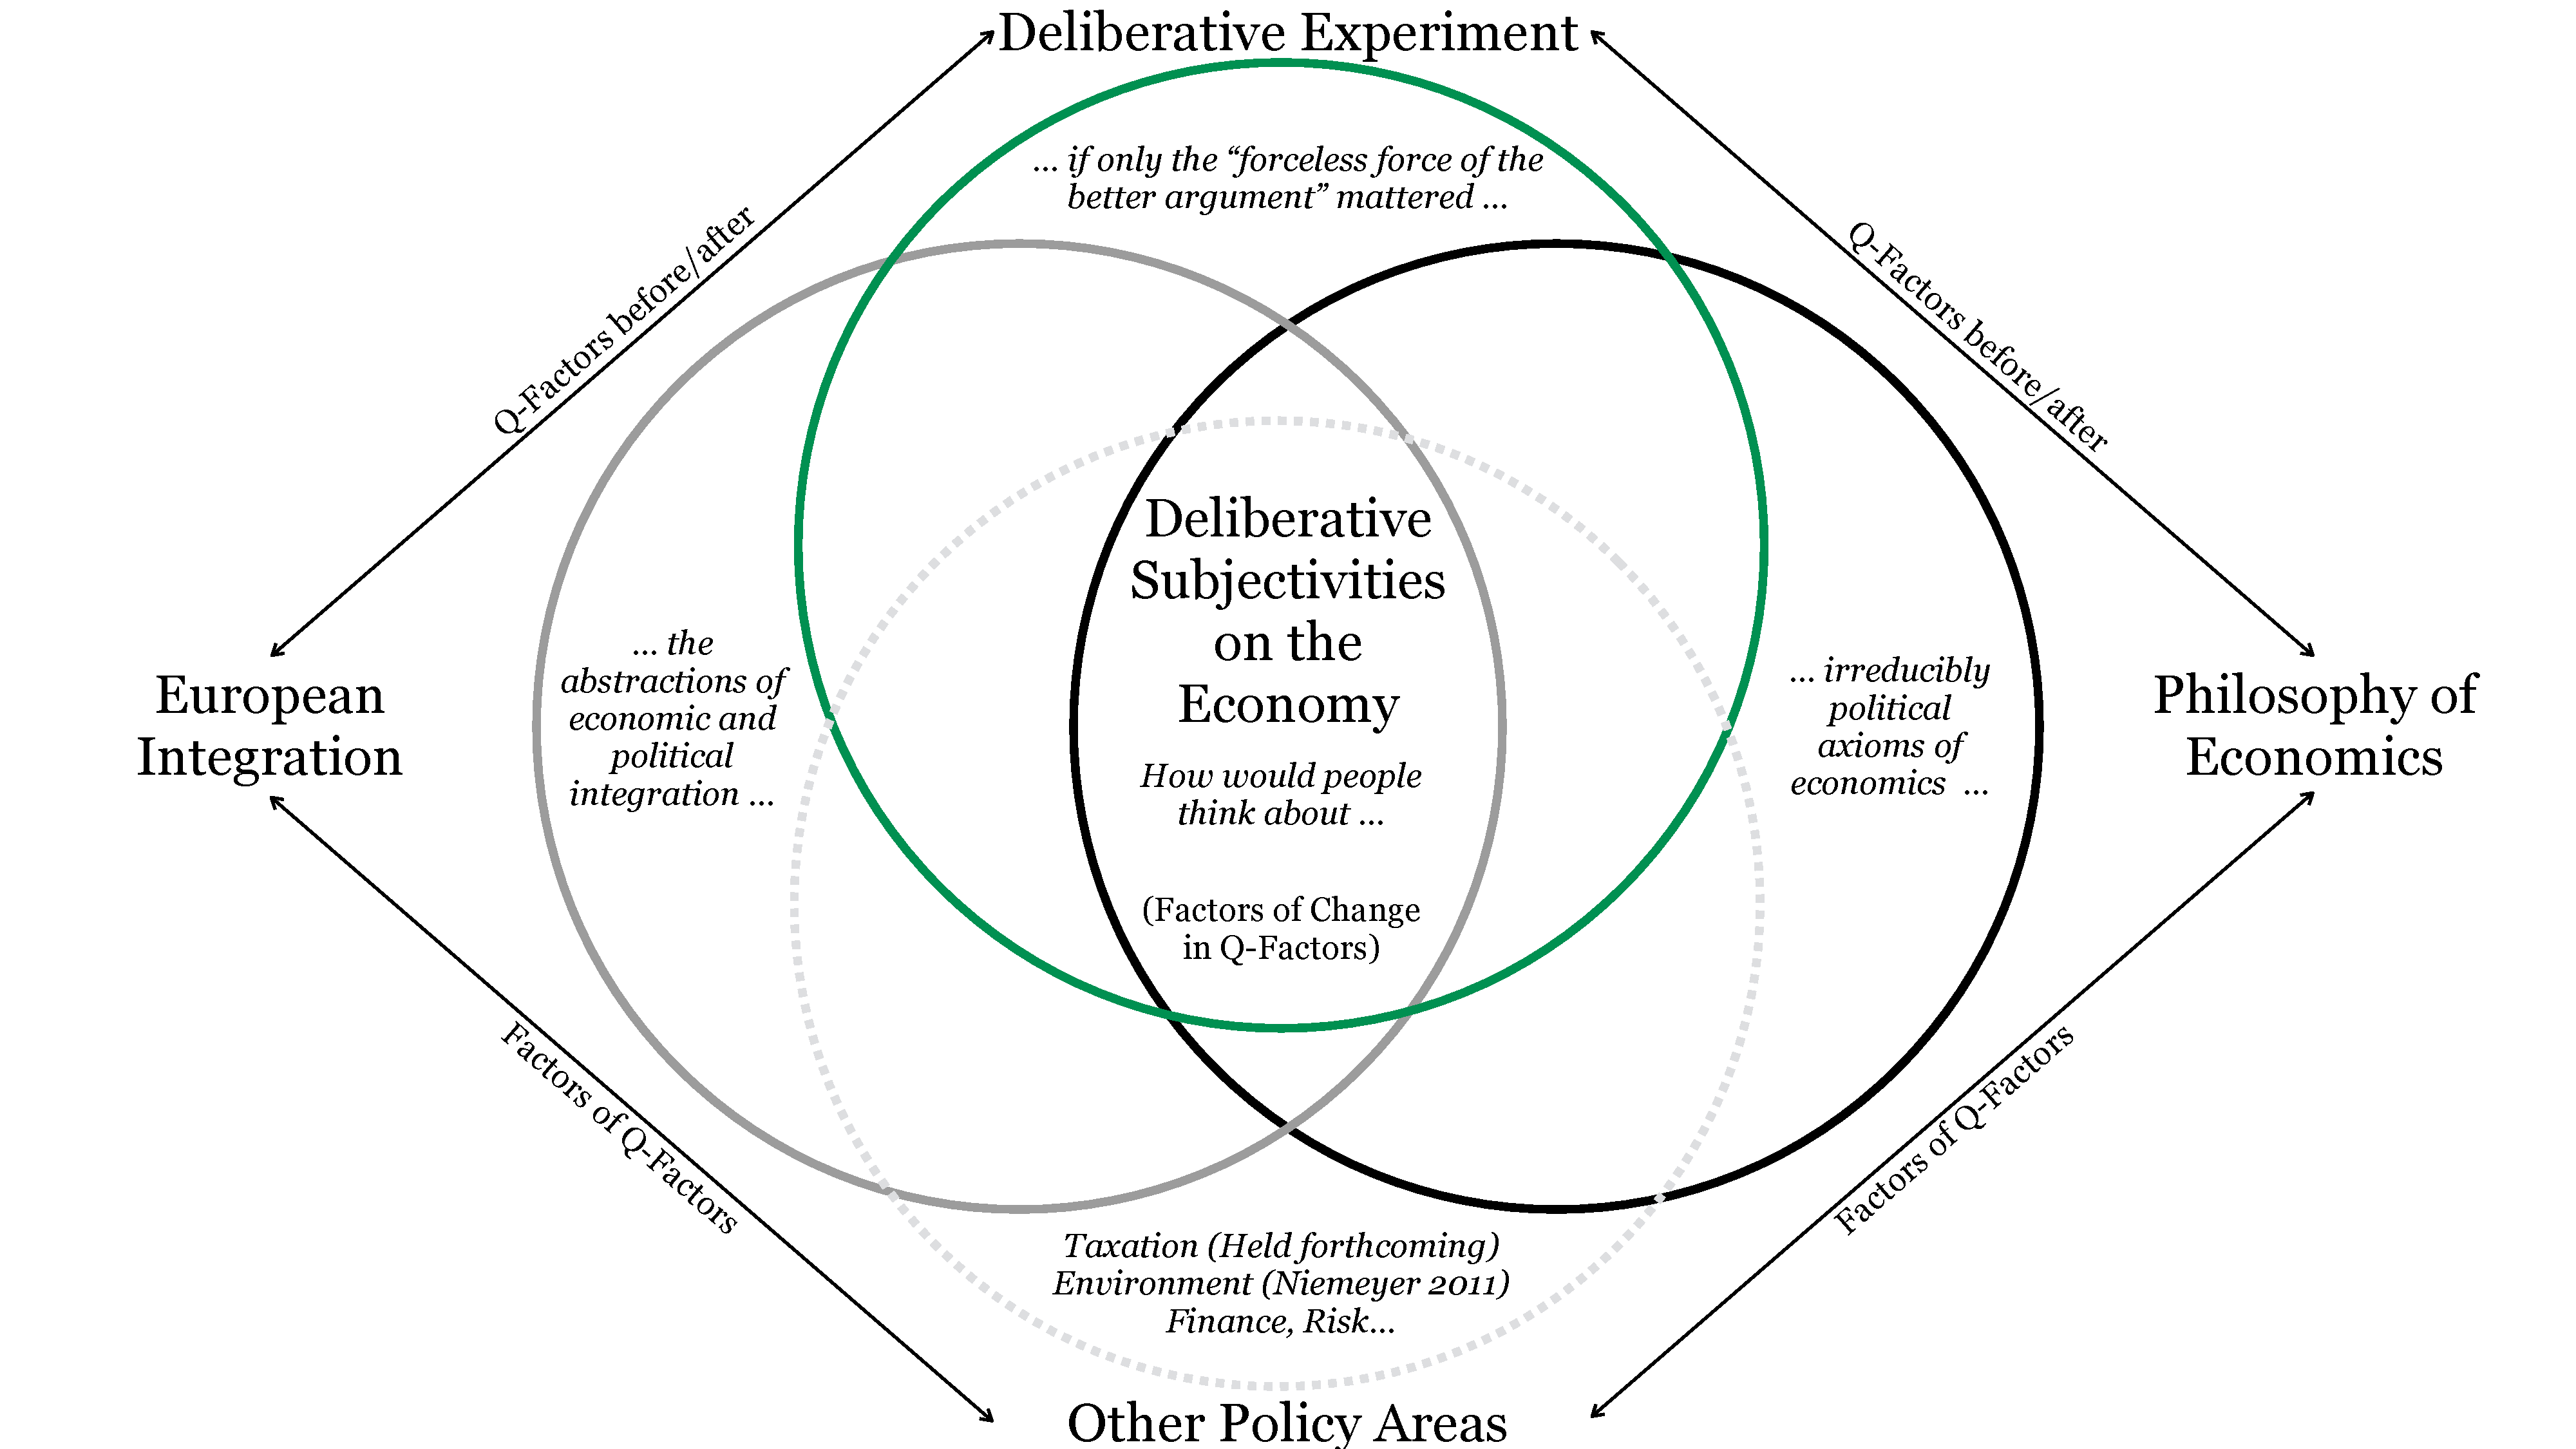
\includegraphics[width=1\linewidth]{img/deliberative-subjectivities}
	\caption{Conceptual Map of the Research Project ``Deliberative Subjectivities on Economic Integration (In the EU)''}
	\label{fig:deliberative-subjectivities}
	\end{center}
\end{figure}
\end{landscape}

\subsection[European Integration]{European Integration as Negative Integration} \label{sec:european-integration}


\paragraph{The European Mixed Economy.}

European welfare states are best understood as mixed economies, where free market exchange is supplemented by planned state command in the service of equity, efficiency, or both \parencite{MusgThet1959}.
In well-designed mixed economies, market and plan co-exist with minimal mutual distortions, and democratic sovereigns can trade off efficiency and equity at relatively small marginal cost \parencite[4]{Bordo2011}.
Intact mixed economies rely on a set of regulatory, monetary and fiscal tools that operate on the same scale as markets \parencite{Samuelson-1954-eu,Samuelson2005}.

In negative integration, markets expand to larger scale, but states remain organized at lower levels, crippling the command tools of the mixed economy.
As a result, democratic sovereigns can no longer take primacy over the economy and any remaining welfare states will be inefficient, inequitable, unsustainable or all.

European integration is negative integration, and much of the 2010ff Euro-crises and the demise of European welfare states can be fruitfully analyzed as defunct mixed economies.

Some of the existing literature on welfare and retrenchment fails to acknowledge the true constraints and alternatives of a mixed economy, and thereby fails to criticize and explain the societal and political choice of negative integration.

The current acquis threatens welfare, and, ultimately democracy and regional integration.
If the EU is to succeed, more economic integration must again always beget more political integration.

%Genschel, too, reminds us of what Pangloss would rather have us forget: “The e↵ect [of globalization] is not so much to force change upon the tax [and thereby, welfare] state as to reduce its freedom to change.” (2005: 53).


%fixes
	%angleichung von faktorpreisen
	%agglomeration and NTT
	%

% Background
% The case (but also more than a case): European Integration
% Compared against an idealised mixed economy, the European Union (EU) displays a sharp imbalance between deeply integrated markets (the common market), but embryonic transnational economic governance. The absence of tax harmonisation, and a union-wide management of aggregate demand (AD) in particular cause unintended market-state interactions. Much of the current sovereign debt and banking crises as well as the resulting economic slump can be understood as the cyclical outgrows of these structural dysfunctions (in addition to microprodutential dysfunctions in financial markets).
% (this diagnosis, admittedly, starts from neoclassical and ordoliberal assumptions; these assumptions themselves need to be problematised; see below meta-theory)
% Behind these crises of an incomplete mixed economy lurk the deeper question of how economic convergence in a starkly unequal union is to be organised, and politically legitimated.

%On this one leg, rergional integration has occured folloing the rolemodel of national economies; the common market guarantees factor (labor, capital) and goods mobility (products, services), effectively regulated by the EP and the Commission.

%european economic order is missing essential institutions of postwar mixed economies; economic integration in the current mode risks the accomplishments of western welfare state, disturbs the historic balance between efficiency and equity goals and creates macroeconomic imbalances which unload in periodic crises.

%negative integration sucks

%assumptions-failures list; look at this also in terms of the disagreement

%problems solutions mixed economy -- does that make sense?

%story about the missing leg, generally
%story of redistribution behind economic integration
%really look at FES; this isn't a european problem, but Europe has always been the project to fix this.

% Gerd Grözinger
	%conflict between economic efficiency and political legitimacy remains (this is the booktitle)

%why go this deep on european questions? because EU integration is the economic modernization question of our age, as maybe, 200 years ago, it was the dissolution of status priviliges.

%What kind of an economic reality results from this open, but heterogeneous EU, with unbounded trade, mis-configured currency union and rampant tax competition?
%BoP logic is important, so is Haig-Simons identity
%aaaand comparison to ideal mixed economy

% Ökonomische Schlussfolgerungen:
% \begin{enumerate}
% 	\item Effiziente und faire wirtschaftliche Integration braucht immer eine \alert{intakte Mischökonomie mit unionsweiten Steuern}.
% 	\item Das Wohlstands- und Produktivitätsgefälle in der EU macht einheitliche Steuersätze einstweilen unmöglich; wir brauchen eine \alert{Transferunion}.
% 	\item Reales Entsparen, Kredit oder Asset-Blasen und Inflation können Krisen verstecken, verschieben und verschlimmern.
% 	\alert{Nichts ist gut, weil nominelle Variablen wie BSP oder Beschäftigung gut aussehen.}
% 	\item Kapitalmärkte mögen bessere Regulierung brauchen; \alert{Finanzkrisen sind aber letztlich Epiphänomene}.
% \end{enumerate}


%second and first order questions

\paragraph{The EU-25 as a defunct mixed economy.}
%tax competition (PD)?

%table assumptions perfect competition

%include dimensions of human need, failures table

%twin crises

%and dual crises links to political system and vice versa

%Democracy needs not just a legitimacy of inputs, but also of outputs (on Europe see Scharpf 1999). In Dahl’s (1994) terms, democracies need to be “system e↵ective”, in Zu ̈rn’s (2000) apt words, democracies need to be “output congruent”: people must be able to choose any (liberal) policy they want to govern a given polity. The EU, currently violates output congruency: with an impotent, largely defunct mixed economy, the people of Europe cannot have all materially possible policies to improve their currently grim life chances, including crushing trade imbalances, demoralizing structural unemployment, wild economic cycles, public squalor and rampant inequality. In the half-built, supposedly sui generis glass of Europe, there is a wide mismatch between the two walls: the exchange components of the mixed economy roam the continent, while most of the command components are confined to the constrained nation state. As a result, the glass is heavily leaking water, both in e

\paragraph{Political Crises}

%[...] that every interim solutions between the extremes of intact national sovereignty on the hand, and complete european supra- nationalty of a European Federation will, inevitably, violate both the reference point of welfare state protection and that of demo- cratic legitimacy.227 — O↵e (1998: 41)

%It does not take another genius to, as Keynes (1936) did in 1918, an- ticipate the economic consequences of this particular peace, and to recog- nize how fragile this mode of one-sided, one-legged, market-only European integration is. It is both the greatest strength and greatest weakness that democracy, to thrive and to persist, must be able to complement market pro- duction and distribution with a plan.

\paragraph{The End Game}
%It also seems a little bit unfair to blame it all on Europe. Negative is the current mode of worldwide economic integration, not just in Europe. The EU and its MS play the same PD games not just on this continent, but on higher levels with other countries. The contradictions of a liberalized world economy without a world government are not merely european problems.

\subsection[Deliberative Experiments]{Experiments Deliberative Democracy} \label{sec:deliberative-experiments}

%table comparing deliberative and aggregative democracy

% The method (but also more than a method): Deliberative Democracy
% The empirical study of deliberative democracy investigates if, and how, people can reach different (more rational?) decisions, if they participate in prolonged, egalitarian, common-good oriented, mutually-understanding discussion.
% Cases: Existing research focuses mostly on local, non-abstract issues (say, waste disposal location), and short formats (half a day).
% Methods: Methodological approaches to studying deliberative democracy fall broadly into two camps; 1) quantitative, survey-type instruments and 2) qualitative, discourse-analytic approaches. Both fall short of approaching a substantive (not merely procedural) standard of deliberation, as espoused by Habermas. Quantitative approaches reduce deliberation to knowledge gain and attitude change (Fishkin), and (critical) discourse analyses put researchers in the awkward position of adjudicating substantive disagreements.
% Niemeyer and Drysek have suggested an attractive, alternative operationalisation of deliberation: good deliberation has happened, when people prefer same policies for the same value- and belief-reasons (and vice versa) (intersubjective rationality), and agree on the realm of alternative preferences, values and beliefs (metaconsensus). This can be measured with Q-Methodology, a (sort-of) inverted factor analysis of sets of around 60-90 statements that participants are asked to rank-order before and after the deliberation, in an experimental setup.

% The political debate (austerity vs profligacy, moral hazard) appears to bear little resemblance to some of the economic abstractions (perfect currency unions, systems competition, etc.) central to understanding these crises.


\paragraph{Misunderstandings}

%include Caplan, that's the guy
%cite the deliberative poll on EU!

%deeper disagreement might play out on economic nationalism ("identity")
	%as well as the definition of "pragmatism" itself, i.e. which stuff you can ask for.
	%In pension design, as elsewhere in public policy, a Haig-Simons understanding of the economy helps us to sift through the epiphenomenal debates (“funded” vs. PAYGO), to relegate the complex details (financial markets) to appropriate theory and data, and advance to those choices that our scarce, constrained and material world leaves us to take: how much we should save for future gen- erations and in which form, and who of us, rich or poor, should contribute how much.

%History of ideas suggests ideas are explanans, what *ought to be explained*; but that's not me, I am somewhere in between and the other position (would that be econ?)


\subsection[Philosophy of Economics]{Philosophy of Economics} \label{sec:philosophy-economics}

% The (meta-?)theory: Philosophy of economics
% Some apparent popular disagreement on economic policy (in EU integration and elsewhere) may be traced to misunderstandings, and lack of knowledge. There is some empirical research on these systematic misunderstandings (McCaffery, Baron), but - as outgrows of prospect theory (Kahnemann/Tversky) - they tend not to cover high-level, abstracted choices.
% However, a substantial core of economic axioms will remain, the validity of which experts cannot adjudicate themselves (i.e.. to what extent is / ought to be / can pragmatically assumed to be / homo sapiens a homo oec.? What is "added value"? etc.). We need to establish plausible links between these low-level axioms and disagreement on policy choices.
% Moreover, these axioms ought to be deconstructed, and then reconstructed by a discerning body of citizens.

%other topic

%explain the alternative first

%vnM rationality link between ordinal preferences and cardinal utility.

%ideal observation Rawls 1998

%copy from the "difference" section of europe

%stress the feat of cooperation, or positive sum gains, literature too; that (in the form of positive economies of scale) is by definition our way out of the Malthusian crises; "this achievement can hardly be overstated"
%the broad question of economic integration that lurks here can hardly be overstated; and not only in the familiar "peace after Weimar" rhetoric; though that works, too.
%enumerate some (preliminary) axiomatic problems with economics:
	%comparative statics is only one, simplistic way to think about it
	%first theorem of welfare economics starts from *given* distributions; that's crucially not the case in Europe
	%

%note the emptyness of economic welfare logic – but what can be put in its place?

% \begin{enumerate}
% 	\item Die Nutzen, Kosten und Bedingungen der wirtschaftlichen Integration müssen \alert{umfassend erklärt} werden.
% 	Zur wirtschaftlichen Integration und dem \alert{Abschied von imaginierten Gemeinschaften} wie dem Nationalstaat gibt es keine attraktive Alternative.
% 	\item Vollbeschäftigung (links, Nachfrageseite) \emph{und} BSP (rechts, Angebotseite) \alert{taugen beide nicht als \emph{hinreichende Ziele} für gute Politik}.
% 	\item \emph{Vielleicht} geht bei wirtschaftlicher Integration \alert{Tiefe vor Breite}.
% \end{enumerate}


% Grundsätzliche alternativen im verstehen der ökonomie; etwa Böll, Institutionenökonomie etc. Etwa eine "europäische dingsda politik" oder die idee des wettbewerbes lassen (im besten Fall) sich zurückführen auf grundsetzlichen dissens, oder totales missverständnis von "unkonzepten", oder eben auf interessierte Ideen (idea research) – but you can't always assume that.

\subsection[Q-Methodology]{Q Methodology} \label{q-methodology}

%concourse sampling strategy for eu, too? (table)

%# Habermas Ach Europa
% so clearly, we want only a notion of a plausible *possibility* of rational solutions, we don't want to look just at rational solutions (first vs second order).
% However, you can't just defer this to process; that would be insufficient, and turn full circle. A deliberation is good if it makes rational solutions plausible, and solutions are plausible if they result from good deliberation. Discuss the different operationalizations about this, including DQI.
% So what we need, is some kind of standard that is not procedural, but also not substantive, but in-between, kinda like  Rawls. But we don't have that ideal position (but we might approximate it?)

% Somehow the stuff that happens during deliberation is actually quite close to some of the stuff that q methodologists rights and that stephenson assumed; it's in expressing and exchanging views vis-a-vis subjects. Both approaches negate that there's stuff "in the braiN" that just need be extracted.

\subsection[Other Policy Areas]{Other Policy Areas} \label{sec:other-policy-areas}

\section[Research Questions]{Research Questions} \label{sec:research-questions}

%there is a deeper research project behind this, for which these different economic cases are, well cases.

% Research question(s) (in increasing levels of abstraction)
% How would ordinary citizens think differently about european integration, if they had the time to thoroughly inform themselves and deliberate amongst one another?
% Can deliberation work on another (like tax) highly complex issue, with (ideally) an international group of participants?
% What is the structure (=rotated factors) of citizen subjectivities on european integration, and how does this structure change as a result of deliberation?
% Building on my previous work on the subjectivities on tax, what are the broader structures of deliberative subjectivities on economics (meta-factors, or factors at the levels of economic axioms?


\section[Project]{Project} \label{sec:project}

The present project tightly integrates teaching, research and outreach and affords several opportunities for cooperation with and around the Europa-Universität Flensburg (EUF), as illustrated in \autoref{fig:euf-partners}.
\footnote{
	From experience, not all such cooperative efforts pan out.
	Intensive cooperation between organisations, individuals and across different interests, in any case, is best organized in person and not at the drawing board.
	Still, this list provides a number of starting points.
}

\textbf{Teaching}, as described in \autoref{sec:teaching} centers around the economics of european integration, its philosophical underpinnings and social-scientific methods for measuring subjectivity.
By linking economic foundations and application, this teaching enables students to criticize EU economic integration on their own terms.
Teaching also serves to \emph{prepare}
 outreach efforts, as students distill preparatory material for citizens from their reading and participate in civics education.
Teaching these seminars also hopes to me \emph{more than preparation}, by practising what deliberative democracy preaches: to argue reasonably disagreing positions on their merits, above and across the ideological fray.

\textbf{Outreach} efforts, as listed in \autoref{sec:outreach}, include civics education for students and long-form deliberative fora for citizens.
These activities constitute the \emph{field work} for the present research on deliberative subjectivites on economic integration and deliver (q-sort) data for analysis and publication.
Outreach is also \emph{more than fieldwork} because these experiments must --- simply for concept validity --- also constitute serious civil society initiatives at citizen participation.

The \textbf{research} component as described in \autoref{sec:research} serves to distill \emph{reasonable disagreements} on economic integration as well as related controversies in the philosophy of economics.
These sets of disagreements are then expanded into preparatory material for citizens during teaching and guide the q-sampling of statements for the fieldwork.
Q-sort data gathered during the fieldwork will then be analysed for common structures (q-factors) of preferences, beliefs and values and their hypothesized change as a function of deliberation.




%not all of these ideas for collaboration will work out; local knowledge always matters, and collaboration is best discussed over a coffe table, not planned at a reissbrett.

%interdisziplinäre Europastudien

%Die Forschung an der Europa-Universität Flensburg konzentriert sich auf die Schwerpunkte Bildung, Wirtschaftswissenschaften, Umweltwissenschaften mit einem Fokus auf den interdisziplinären Bereich Nachhaltige Entwicklung und interdisziplinäre Europastudien. [website]
	%bingo; genau in der Schnittmenge liegt das Projekt

%mit lehrerbildung kooperieren. – als pilotprojekt, und um die didaktische Konzeption zu schärfen
	%EULE - lehrerbildung
	%welche fachbereiche in der lehrerbildung gibt es?
	%pilotversuche an Partnerschulen
	%im unterschied zu gegenwärtiger Europaschulung geht es *nicht* um institutionkunde, sondern um die (ökonomischen) Abstraktionen der Einigung
	%Vergleich auch Eurolektionen!
	%Drittmittel evtl. aus Horizon 2020
	%Bürger-krams:
		%http://hhsh.enterprise-europe-germany.de/public/uploads/een-hhsh/downloads/KurzinfoEuropafuerBuergerInnen.pdf
	% some kinds of venn diagrams with european integration, mixed economy, philosophy of economics, deliberative subjectivities of the economy in the center
	% also diagram with inputs, outputs etc.
	%also diagram: (maybe downward thing, links ziel / Rechts geldgeber etc.
		%1. FORSCHUNG Europa als (dys)funktionale Mischwirtschaft
		%2. LEHRE forschendes lernen / gemeinsames schreiben
			%Studiengang MA European Studies
			%Studiengang MA Intl Management
			%Studiengang FH: wirtschaftsinfo?
			%Studiengang BA Bildungswissenschaften / MA Ed Gemeinschaftsschule\tabularnewline
			%Gesellschaftswissenschaften, ABER AUCH AESTHETISCHE BILDUNG!
			%vorhab github-schulung
			%verweis auf forschendes lernen der studierenden (lehrer) von der TITTF.
			%SEMINAR: schreiben auf GIT/LATEX?!
			%SEMINAR: q-methode und andere empirische sozialforschung / umfragen
			%SEMINAR: Mischwirtschaft etc. (2 Semester, ggfs, mit Mikro- Makro einführung erforderlich)
		%3. PROJEKT an lokalen Schulen (eurolektionen)
		%4. LEHRERBILDUNG
			%fachdidaktik Wirtschaft, Politik, Europa
		%5. CIVICON
		%6. FORSCHUNG: Q-Studien abgreifen
		%auch aufschreiben: Planspiele, weitere didaktische Übungen, sowie TANZEN etc.
%Institut für Ästhetisch-Kulturelle Bildung
%Institut für Erziehungswissenschaften:
	%darin vor allem Schulbildung
%Institut für Gesellschaftwissenschaften und Theologie
	%Seminar für Politikwissenschaft und Politikdidaktik
	%Seminar für Geschichte und Geschichtsdidaktik
%Internationales Institut für Management und ökonomische Bildung
	%Abteilung Wirtschaftswissenschaften und ihre Didaktik
	%Abteilung Sozial- und Bildungsökonomie
	%Abteilung Internationale und Institutionelle Ökonomik
	%Abteilung Finanzwirtschaft
	%Abteilung Europa- und Völkerrecht
%Interdisziplinäres Institut für Umwelt-, Sozial- und Humanwissenschaften
	%darin vor allem Abteilung Zentrale Methodenlehre
%Kooperationsschulen an der Uni Flensburg
%Zentrum für Lehrerbildung?
%vielleicht als interdisziplinäres Projekt im Rahmen des Master of Education (Gemeinschaftsschule)

\begin{landscape}
 \begin{figure}[htbp]
    \begin{center}
	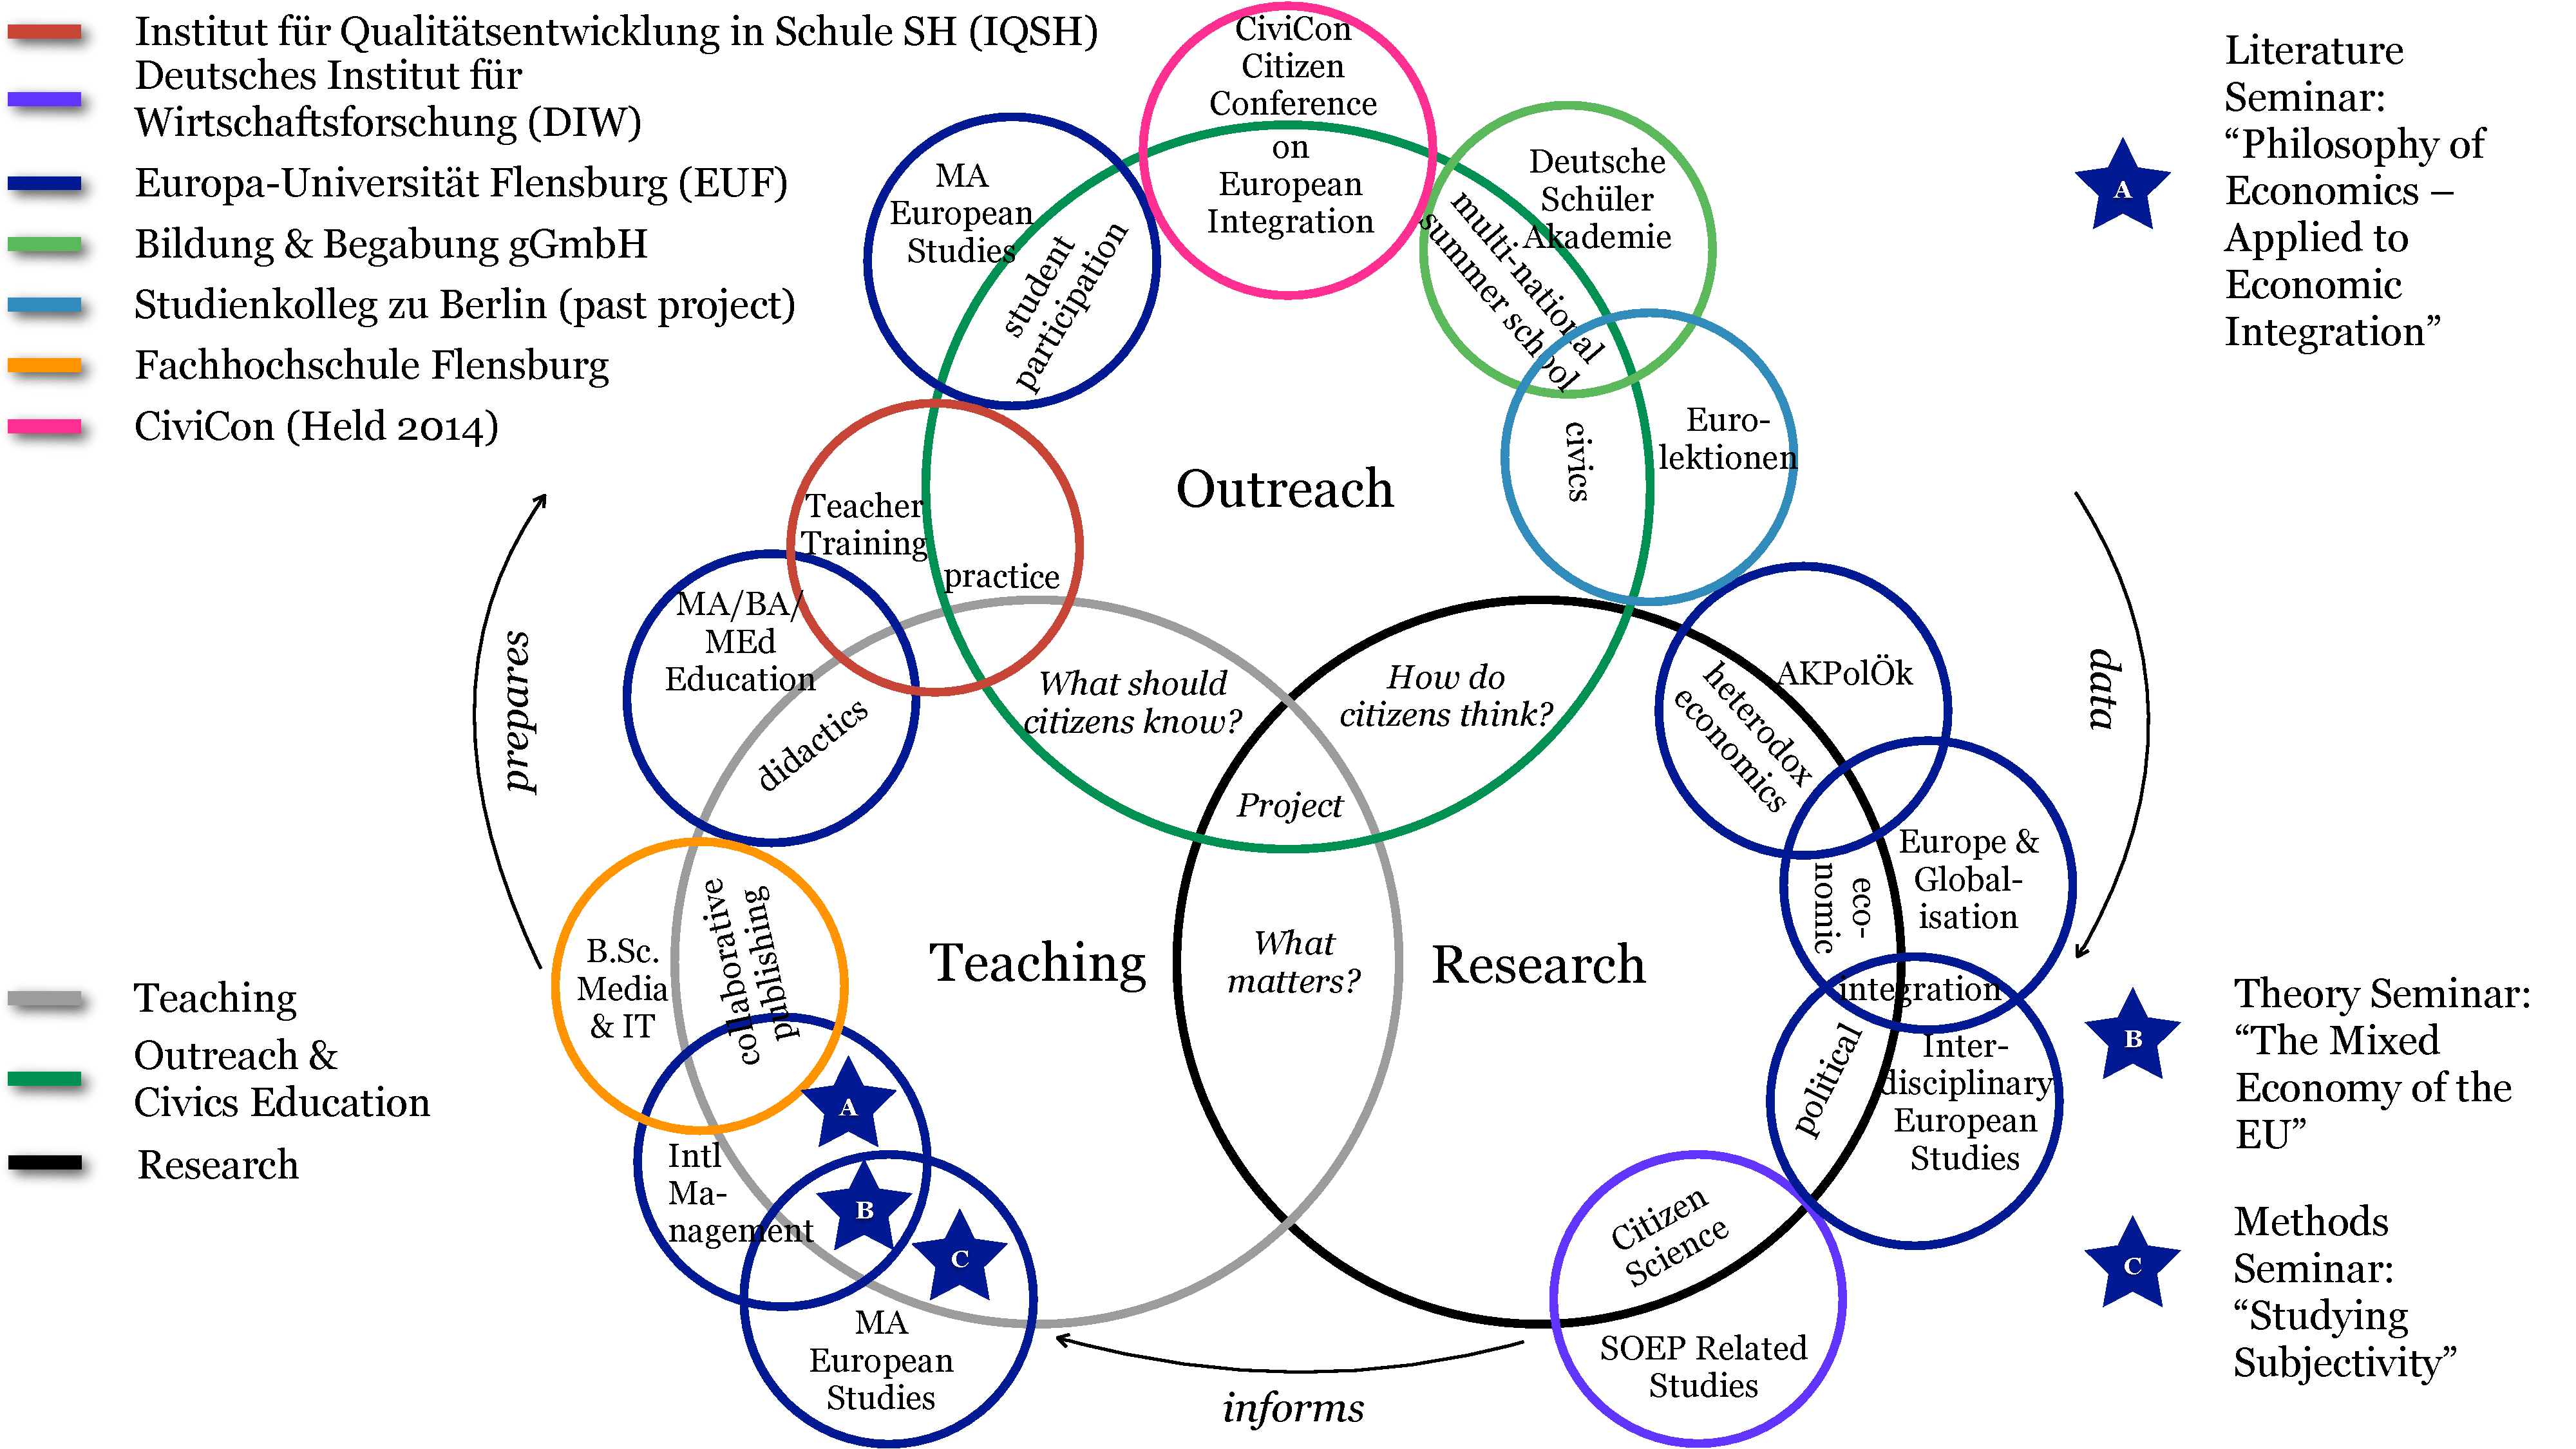
\includegraphics[width=1\linewidth]{img/euf-partners}
	\caption{Possible Cooperation Partners for Research Project}
	\label{fig:euf-partners}
	\end{center}
\end{figure}
\end{landscape}

\subsection[Teaching]{Teaching} \label{sec:teaching}

% Project components / Links to EUF
% Teaching
% (2-semester) literature seminars (in MA European Studies / MA Intl Management / MA Lehramt Mittelschulen)
% Intensive theory reading; philosophy of economics as applied to the economics of regional integration.
% Collaborative writing (via GitHub / LaTeX) of a handbook for citizens: what are the most important and most controversial abstractions people have to know about regional (EU) integration?
% Pre-Testing of Q-Sorts (students will complete q-sorts before and after their seminar participation)
% (extent/format of this course will depend on prerequisites, ideally Micro-/Macro-Economics, as well as institutional economics – may also be opened for interested BA students)
% (1-semester) methods seminar (in MA European Studies, MA Intl Management, MA Lehramt Mittelschulen)
% review of mainstream empirical social research methods
% how does q-methodology compare?
% development, analysis of q-sample
% (1-semester) didactics seminar (in MA Lehramt Mittelschulen)
% collaboration with teacher education at EUF
% how can the economics of european integration be taught to diverse, international groups following deliberative standards?

\subsection[Outreach]{Outreach \& Civics Education} \label{sec:outreach}

% Civil Society Outreach ("Politische Bildung"):
% School project on European integration with local schools, and student teachers (model: Eurolektionen from 2009)
% ideally with danish students, too.
% serves as pre-test with focus on didactics
% cooperation with Lehrerbildung / EULE @ EUF
% limited (internal?) funding required
% Summer school with 16-20 year olds (model: Deutsche SchülerAkademie)
% with german students
% 2 weeks
% serves as pre-test with focus on didactics
% limited (internal?) funding required
% may be scaled up to international summer school, would require substantial funding
% CiviCon on European Integration (model: CiviCon on Taxation)
% A citizen conference on european integration, 2-4 weeks
% ideally with european participants
% would require substantial (external!) funding

\subsection[Research]{Research} \label{sec:research}

% Publication opportunities from development of handbook, and literature review of philosophy of economics as applied to economic integration in the EU.
% Publication opportunities from iterative administration of q-sorts to students.
% Preparation and acquisition of substantial funding for a CiviCon on European Integration.
% Development of a research project into the deliberative subjectivities on economics.


\section[Job Profile]{Job Profile} \label{sec:job-profile}

%Q method
%deliberation
%teaching
%economics

\printbibliography
\end{document}